\section{Conclusion}

\begin{frame}[t]{Conclusion}
  \visible<1>{
    \picpos{.3\linewidth}{0cm}{3cm}{tunable_laser.jpg}
    \picpos{.3\linewidth}{.3\linewidth+0.2cm}{2.5cm}{ion_trap.pdf}
    \picpos{.3\linewidth}{0.6\linewidth+0.4cm}{3cm}{cavity_photo.jpg}
  }
  \begin{itemize}
    \item<1-> Possible only with tunable lasers, ion traps and semiconductor
      technology
    \item<2-> observation of single particles for fundamental insight into
      principles of quantum mechanics:
      \begin{itemize}
        \item quantum jumps
        \item entangled states
        \item decoherence processes
      \end{itemize}
    \item<3-> possible applications in quantum computing (e.g. Q20:20)
    \item<4> a decent set of experimental methods for future physicists to play
      with
  \end{itemize}
\end{frame}

\begin{frame}[t]{Take home message}
  \begin{center}
    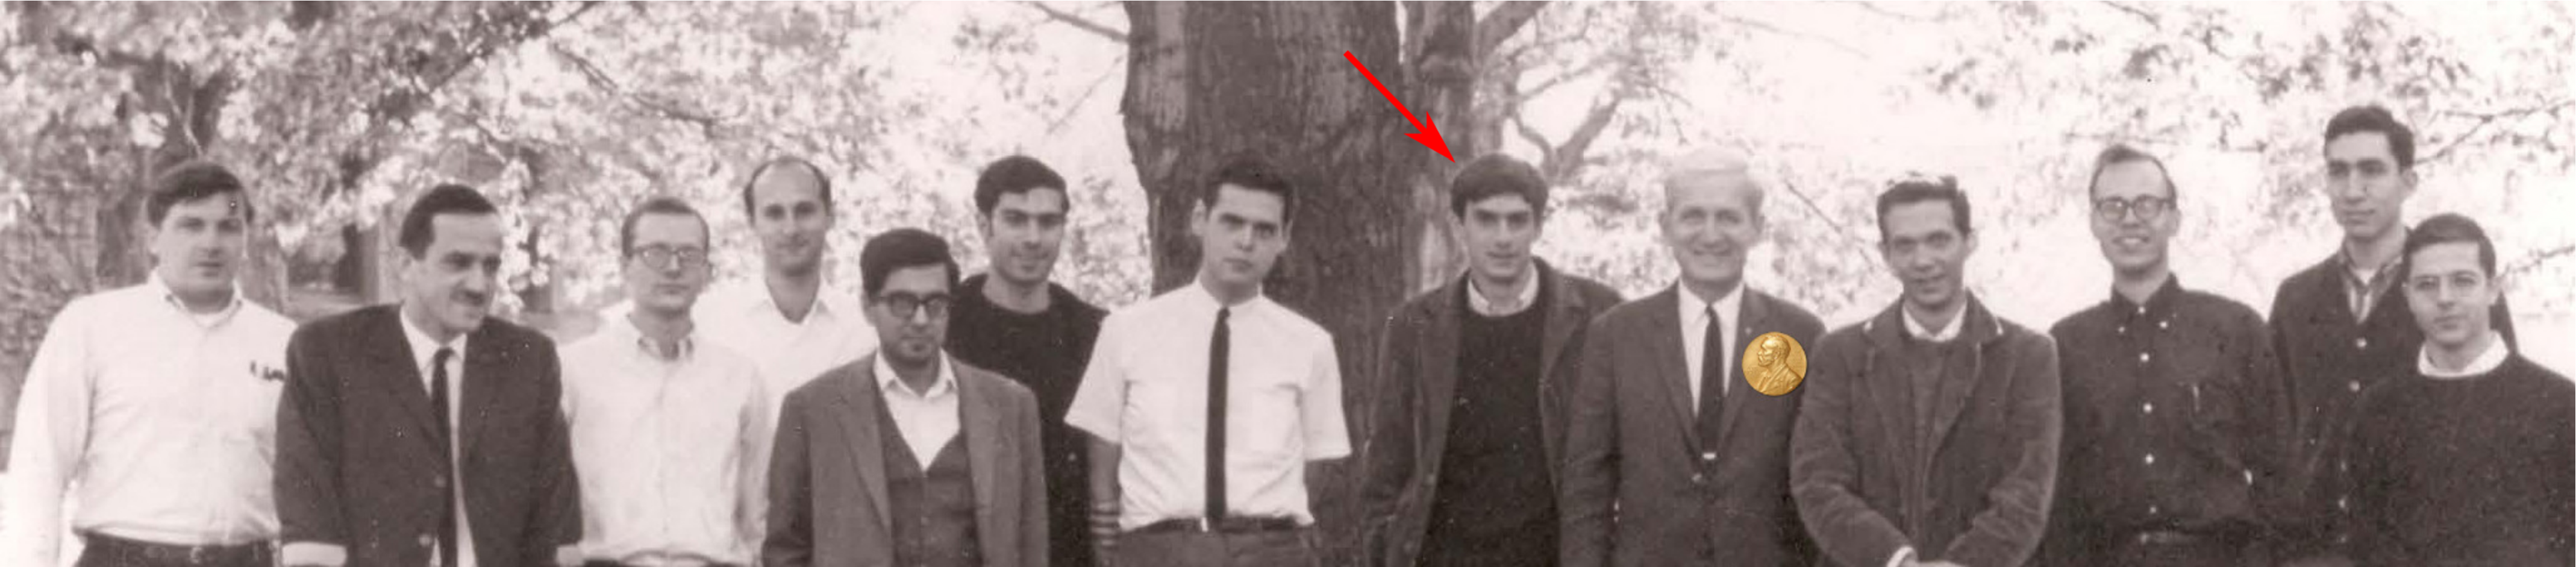
\includegraphics[width=0.9\textwidth]{norman_ramsey_group_arrow.pdf}\\
    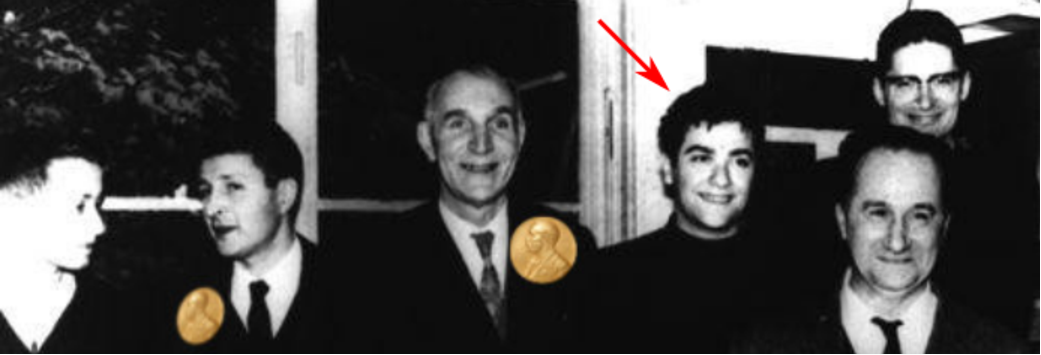
\includegraphics[width=0.9\textwidth]{lab_kastler_arrow.pdf}\\
    \vspace{0.1cm}
    If you plan on winning a nobel prize, try to stand next to your
    future-nobel-laureate-supervisor during your PhD
  \end{center}

\end{frame}
